\section{Question 5}

\begin{question}
    Analyze the Correlation Matrix to discover pairwise correlations between data attributes. Report a
screenshot showing the correlation matrix achieved.
    \\
    (a) Does the Naïve independence assumption actually hold for the Breast dataset?
    \\
    (b) Which is the pair of most correlated attributes?
\end{question}

\begin{answer}
    a: The correlation matrix shown on figure 11 shows that there are many correlated
    attributes. Therefore the assumption does not hold.
    b: The pair most correlated is inv-nodes and node-caps, which is actually inversely
    correlated, followed by inv-nodes and irradiat pair, which is directly correlated.
    \begin{figure}
        \centering
        \subfigure[]{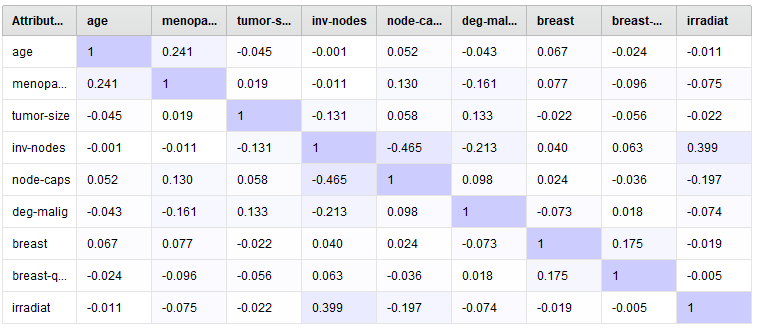
\includegraphics[width=0.48\textwidth]{Screenshot_30.png}}
        \caption{Correlation matrix}
    \end{figure}
    \begin{figure}
        \centering
        \subfigure[]{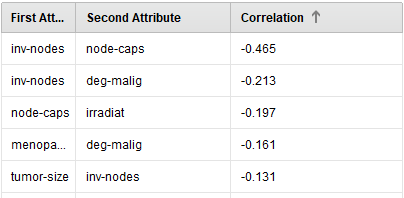
\includegraphics[width=0.48\textwidth]{Screenshot_32.png}}
        \caption{Top inversely correlated fields}
    \end{figure}
    \begin{figure}
        \centering
        \subfigure[]{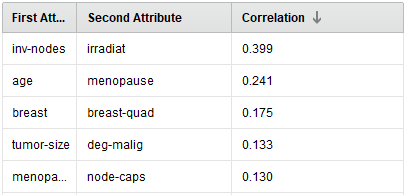
\includegraphics[width=0.48\textwidth]{Screenshot_31.png}}
        \caption{Top directly correlated fields}
    \end{figure}
\end{answer}
